\section{Final Obstacle: \texorpdfstring{$f_8$}{f8}}
\label{sec: 2n=8}
\label{sec: f8}

In this section, we will complete the induction proof for $2n=8$  (\cref{thm: base case 2n=8}).
We assume that $\mathcal F$ does not satisfy condition \rm{(\ref{cond: tractable classes})}, and $\mathcal{F}$ contains a signature $f\notin \mathcal{U}^\otimes.$

Shao and Cai discovered the signature $f_8$ in \cite{realholant}.
It is $f_8=\chi_C$ where
\begin{equation}\label{eq: f8}
 \begin{aligned}
  C=&\mathscr{S}(f_8)=\{(x_1, x_2, \ldots, x_8)\in \mathbb{Z}_2^{8} \mid~
x_1+x_2+x_3+x_4= 0, ~ x_5+x_6+x_7+x_8= 0,\\
  &\hspace{34ex}x_1+x_2+x_5+x_6= 0, ~ x_1+x_3+x_5+x_7= 0\}.\\
=&\{00000000, 00001111, 00110011, 00111100, 01010101, 01011010, 01100110, 01101001,\\
& ~10010110,  10011001, 10100101, 10101010, 11000011, 11001100, 11110000, 11111111\}.
\end{aligned}
\end{equation}

$f_8$ have some extraordinary properties.
For example, it satisfies {\sc 2nd-Orth} and $f_8\in \int \mathcal{U}^{\otimes}$.
Thus, simple merging and factorization cannot realize a signature outside $\mathcal{U}^{\otimes}$.
In \cref{subsec: realize f8 Reed Muller}, we will realize $f_8$.
In \cref{subsec: f8 available hardness}, we prove \#P-hardness when $f_8$ is available.

\subsection{Realizing \texorpdfstring{$f_8$}{f8} Through the Lens of Reed-Muller Code}
\label{subsec: realize f8 Reed Muller}

\begin{definition}[Strong equality property]\label{def: Strong equality property}
    Let $\mathcal{E}^\otimes=\{\lambda\cdot (=_2)^{\otimes n}\mid \lambda\in \mathbb{C}^\times,n\ge1\}$ be the set of tensor products of binary $=_2$ up to a non-zero scalar.
    We say a signature $h$ satisfies the \emph{strong equality property}, if $h\in \int \mathcal{E}^{\otimes}$, i.e., for any pair of indices $\{i,j\}$, $\partial_{ij}h\in \mathcal{E}^\otimes.$
\end{definition}

It can be checked that $f_8$ satisfies the strong equality property.
The following lemma is essentially the same as
\cite[Lemma~8.1]{realholant}.
The only difference is that when doing binary extension, we use the conjugate transpose of the binary instead of the binary itself.

\begin{lemma}
\label{lm: unitary wire normalization}
Let $f\notin \mathcal{U}^\otimes$ be a signature of arity $2n\ge 8$ in $\mathcal{F}$.
Then one of the following holds:
\begin{itemize}
    \item $\Holant(\mathcal{F})$ is \#P-hard;
    \item There is a signature $g\notin \mathcal{U}^\otimes$ of arity $2k\le 2n-2$ that is realizable from $f$;
    \item There is an irreducible signature $f^\ast$ of arity $2n$ that is realizable from $f$ with the strong equality property.
\end{itemize}
\end{lemma}

\begin{proof}
Since ${f}\notin {\mathcal{U}}^{\otimes}$, $ f\not\equiv 0$.
Again, we may assume that ${f}$ is irreducible.
Otherwise, by factorization, we can realize a nonzero signature of odd arity and we get \#P-hardness by \cref{lm: odd holant with conjugation}, or we can realize a signature of lower even arity that is not in $\mathcal{U}^{\otimes}$ and we are done.
Under the assumption that $f$ is irreducible, we may further assume that $f$ satisfies {\sc 2nd-Orth} by \cref{lm: not 2nd-orth is hard}.
Consider signatures ${\partial}_{ij}{f}$ for all pairs of indices $\{i, j\}$. 
If there exists a pair $\{i, j\}$ such that ${\partial}_{ij}{f}\notin {\mathcal{U}}^{\otimes}$, then let ${g}={\partial}_{ij}{f}$, and we are done.
Thus, we may also assume that ${f}\in {\int}{\mathcal{U}}^{\otimes}$.  

Since $f$ satisfies {\sc 2nd-Orth}, $\partial_{ij}f$ is non-zero by \cref{lm: 2nd-orth contraction nonzero}.
Since $ {\partial}_{12} {f} \in  {\mathcal{U}}^{\otimes}$, without loss of generality, we may assume that in the UPF of $ {\partial}_{12} {f}$, variables $x_3$ and $x_4$ appear in one  binary signature $b_1(x_3, x_4)$, $x_5$ and $x_6$ appear in one binary signature $b_2(x_5, x_6)$ and so on. 
Thus, we have 
\begin{equation*}
 {\partial}_{12} {f}=   {b_1}(x_3, x_4)\otimes  {b_2}(x_5, x_6)\otimes {b_3}(x_7, x_8)\otimes \ldots \otimes  {b_{n-1}}(x_{2n-1}, x_{2n}).
\end{equation*}

All these binary factors $b_1,b_2,\ldots,b_{n-2}$ are realizable by
\cref{lm: decomposition}.  
Put $B_i=M(b_i)$.  
Since
$b_i\in\mathcal U$ and $b_i\neq 0$, $B_i$ is projectively unitary.  Reversing the two arguments gives $B_i^{\mathtt T}$, and conjugate closure gives
$\overline B_i$.  
Hence the binary signature $b_i^{-1}$ with matrix $B_i^{-1}\propto \overline{B_i}^{\tt T}$ is also available.
We consider the following gadget construction on $f$.
For $1\leqslant i\leqslant n-1$, by a slight abuse of names of variables, we connect the variable $x_{2i+1}$ of $f$   
with the variable $x_{2i+2}$ of $  {b^{-1}_{i}}(x_{2i+1}, x_{2i+2})$. 
We get a signature $f'$ of arity $2n$. 
We denote this gadget construction by $G_1$ and we write $f'$ as $G_1 \circ f$.
$G_1$ is constructed by extending variables of $f$ using binary signatures realized from ${\partial}_{12}{f}$. 
It does not change the irreducibility of $f$.  
Thus, $f'$ is irreducible since $f$ is irreducible.
Similarly, we may assume that $f'\in {\int}  {\mathcal{U}}^{\otimes}$. Otherwise, we are done.


Consider the signature ${\partial}_{12}{f'}$. 
Since the above gadget construction $G_1$  does not touch variables $x_1$ and $x_2$ of $f$, $G_1$
commutes with the merging gadget ${\partial}_{12}$. 
Thus, ${\partial}_{12}{f'}$ can be realized by performing the gadget construction $G_1$ on ${\partial}_{12}{f}$, which connects each binary signature ${b_{i}}(x_{2i+1}, x_{2i+2})$ in the UPF of ${\partial}_{12}{f}$ with  ${b^{-1}_{i}}(x_{2i+1}, x_{2i+2})$. 
Thus, each binary signature ${b_{i}}$ in ${\partial}_{12}{f}$ is canceled up to a nonzero scalar after this gadget construction $G_1$. 
After normalization and renaming variables, we have 
\begin{equation}\label{eqn:lm5-partial12-f}
{\partial}_{12}{f'}= (=_2)(x_3, x_4)\otimes (=_2)(x_5, x_6)\otimes \ldots \otimes (=_2)(x_{2n-1}, x_{2n}).
\end{equation}
Thus, ${\partial}_{12}{f'}\in {\mathcal{E}}^{\otimes}$.
Moreover, for all pairs of indices $\{i, j\}$ disjoint with $\{1, 2\}$,
we have 
\begin{equation}\label{equ-ij-12-in-D}
    {\partial}_{(ij)(12)}{f'}\in {\mathcal{E}}^{\otimes}, \text{ ~and hence~ } {\partial}_{(ij)(12)}{f'}\not\equiv 0.
    \end{equation}
A fortiori, for all pairs of indices $\{i, j\}$ disjoint with $\{1, 2\}$, ${\partial}_{ij}{f'}\not\equiv 0$.

Next, we show that we can realize an irreducible signature $f^\ast$ of arity $2n$ from ${f'}$ such that ${f^\ast}$ has the strong equality property.
We first prove the following claim.

\begin{claim}\label{claim: strong equality property}
    Let ${h}\in {\int}{{\mathcal{U}}}^{\otimes}$ be a signature of arity $2n\geqslant 8$. 
    If $\partial_{ij}{h}$ is a tensor product of $=_2$ up to a non-zero scalar for all $\{i, j\}$ disjoint with $\{1, 2\}$, then ${h}$ has strong equality property.
\end{claim}

\begin{claimproof}{\cref{claim: strong equality property}}
    Clearly, we only need to show that ${\partial}_{1k}{h}\in {\mathcal{E}}^{\otimes}$ for all $2 \leqslant k \leqslant 2n$. Then, by symmetry we also have ${\partial}_{2k}{h}\in {\mathcal{E}}^{\otimes}$ for $k=1$ and all $3 \leqslant k \leqslant 2n$. This will prove ${h}\in {\int}{\mathcal{E}}^{\otimes}.$
    Consider ${\partial}_{1k}{h}$ for an arbitrary $2\leqslant k \leqslant 2n$.
   Since for all $\{i, j\}$ disjoint with $\{1, 2\}$, we have
    ${\partial}_{ij}{h}\in {\mathcal{E}}^{\otimes}$, a fortiori
    for all  $\{i, j\}$ disjoint with $\{1, 2\} \cup \{k\}$,
    \begin{equation}\label{eqn:partial-1kj-in-sec8}
    \partial_{(1k)(ij)}{h}\in {\mathcal{E}}^{\otimes}.
   \end{equation}
    Since ${h}$ has arity $2n\geqslant 8$, we can pick a pair of indices $\{i, j\}$ disjoint with $\{1, 2\} \cup \{k\}$.
    Since $\partial_{(1k)(ij)}{h}\in {\mathcal{E}}^{\otimes}$, which is nonzero,  a  fortiori  we have
    ${\partial}_{1k}{h} \not \equiv 0$.
    So we may consider  the UPF of ${\partial}_{1k}{h}$,
    which is known to be in ${\mathcal{U}}^{\otimes}$.
    For a contradiction,
    suppose that  there is a binary signature  ${b_1}$ (as a factor of ${\partial}_{1k}{h}$) such that ${b_1}$ is not an associate of $=_2$. 
    Among the two variables in the scope of ${b_1}$,  at least one is not $x_2$. 
    We pick such a variable $x_s$ where $x_s \neq x_2$. 
    Then, we consider another binary signature ${b_2}$ in the UPF of ${\partial}_{1k}{h}$. 
    \begin{itemize}
        \item 
    If ${b_2} =\lambda \cdot (=_2)$, for some  nonzero scalar
    $\lambda$, then we pick a variable $x_t$ in the scope of ${b_2}$ that is not $x_2$. 
    Consider ${\partial}_{(st)(1k)}{h}$. 
    When merging variables $x_s$ and $x_t$ of ${\partial}_{1k}{h}$, 
    we connect the variable $x_s$ of  ${b_1}$ with the variable $x_t$ of $\lambda  \cdot (=_2)$, and the resulting binary signature is just $\lambda \cdot{b_1}$, which is not an associate of $=_2$. 
    Thus, we have ${\partial}_{(st)(1k)}{h}\notin {\mathcal{E}}^{\otimes}$.
    
    \item Otherwise,  ${b_2}$ is not an associate of $=_2$. Since ${\partial}_{1k}{h}$ has arity $2n-2\geqslant 6$, we can find another binary signature ${b_3}$ in the UPF of ${\partial}_{1k}{h}$. 
    We pick a variable $x_t$ in the scope of ${b_3}$ that is not $x_2$. 
    Consider ${\partial}_{(st)(1k)}{h}$. 
    Now, when merging variables $x_s$ and $x_t$ of ${\partial}_{1k}{h}$, 
    the binary signature ${b_2}$ is untouched. 
    Thus, we have ${b_2}\mid {\partial}_{(st)(1k)}{h}$, which implies that ${\partial}_{(st)(1k)}{h}\notin {\mathcal{E}}^{\otimes}$.
   \end{itemize}
   
   Note that in both cases, $\{s,t\} \cap (\{1,2\} \cup \{k\}) = \emptyset$. Therefore
   the two cases above both contradict
   (\ref{eqn:partial-1kj-in-sec8}) by picking $\{i, j\}=\{s, t\}$.
      Thus, ${\partial}_{1k}{h}\in {\mathcal{E}}^{\otimes}$ for all $2 \leqslant k \leqslant 2n$. Then similarly, we can show that ${\partial}_{2k}{h}\in {\mathcal{E}}^{\otimes}$ for all $3 \leqslant k \leqslant 2n$. 
\end{claimproof}

Remember that ${\partial}_{ij}{f'}\not\equiv 0$ for all $\{i, j\}$ disjoint with $\{1, 2\}$.
We consider the UPF of ${\partial}_{ij}{f'}$. Since ${f'}\in {\int}{\mathcal{U}}^{\otimes}$, there are two cases depending on whether variables $x_1$ and $x_2$ appear in one  binary signature or two distinct binary signatures.

\vspace{1ex}
\noindent{\bf Case 1.}
    For every $\{i, j\}$ disjoint with $\{1, 2\}$, in the UPF of ${\partial}_{ij}{f'}$, $x_1$ and $x_2$ appear in one nonzero binary signature
    %%% nonzero because the {\partial}_{ij}{f'} is nonzero.
    ${b_{ij}}(x_1, x_2) \in {\mathcal{U}}$.  %If $x_1$ and $x_2$ appear in one single binary ${b}(x_1, x_2)$, 
    In other words, for every $\{i, j\}$ disjoint with $\{1, 2\}$, $${\partial}_{ij}{f'}={b_{ij}}(x_1, x_2)\otimes {g_{ij}}, ~~\text{ for some } {g_{ij}}\not\equiv 0.$$
    (These factors ${b_{ij}}$ and $ {g_{ij}}$ are nonzero since ${\partial}_{ij}{f'}\not\equiv 0$.)
   % those are nonzero because  ${\partial}_{(12)(ij)}{f'}={\partial}_{(ij)(12)}{f'}\in {\mathcal{E}}^{\otimes}$, 
  % and  from (\ref{eqn:lm5-partial12-f}),  it is nonzero. And so we have
  Then, ${g_{ij}} \sim {\partial}_{(12)(ij)}{f'}$, and by
    (\ref{equ-ij-12-in-D}), we have ${g_{ij}}\in{\mathcal{E}}^{\otimes}$. 
    %As a consequence, we have ${\partial}_{(st)(ij)}{f'}\not\equiv 0$.
    Also for $\{k, \ell\}$ disjoint with both $\{i, j\}$
    and $\{1, 2\}$, ${\partial}_{(k\ell)(ij)}{f'}
    \not \equiv 0$ since
    %{\partial}_{k \ell} {g_{ij}}
    %\sim 
    ${\partial}_{(12)(k \ell)(ij)} {f'} = {\partial}_{(ij)(k \ell)(12)} {f'} 
    \not \equiv 0$.
    
    We first show that for any two pairs $\{i, j\}\neq \{k, \ell\}$ that are both disjoint with $\{1, 2\}$,
    ${b_{ij}}(x_1, x_2)\sim {b_{k\ell}}(x_1, x_2)$. 
    If $\{i, j\}$ is disjoint with $\{k, \ell\}$, then  ${b_{ij}}(x_1, x_2)\mid {\partial}_{(k\ell)(ij)}{f'}$ and ${b_{k\ell}}(x_1, x_2)\mid {\partial}_{(ij)(k\ell)}{f'}$. 
    Since ${\partial}_{(k\ell)(ij)}{f'}={\partial}_{(ij)(k\ell)}{f'}\not\equiv 0$, by \cref{unique}, 
    we have ${b_{ij}}(x_1, x_2)\sim {b_{k\ell}}(x_1, x_2)$. 
    Otherwise, $\{i, j\}$ and $\{k, \ell\}$ are not disjoint. Since ${f'}$ has arity $\geqslant 8$, we can find another pair of indices $\{s, t\}$ such that it is disjoint with $\{1, 2\}\cup \{i, j\} \cup \{k, \ell\}$. 
    Then, by the above argument, we have ${b_{ij}}(x_1, x_2)\sim {b_{st}}(x_1, x_2),$ and  ${b_{st}}(x_1, x_2)\sim {b_{k\ell}}(x_1, x_2).$
    Thus, ${b_{ij}}(x_1, x_2)\sim {b_{k\ell}}(x_1, x_2).$
    We can use a binary signature ${b}(x_1, x_2)$  to denote these binary signature ${b_{ij}}(x_1, x_2)$ for all $\{i, j\}$ disjoint with $\{1, 2\}$. 
    Then, ${b}(x_1, x_2) \mid {\partial}_{ij}{f'}$ for all $\{i, j\}$ disjoint with $\{1, 2\}$. 
    Also,  ${b}(x_1, x_2)$ is realizable  from $ f'$ by merging and factorization.
    Then $b^{-1}(x_1,x_2)$ is realizable by taking conjugation and renaming the two variables in $b.$
    
    Then, we consider the following gadget construction $G_2$ on ${f'}$. 
    By a slight abuse of variable names, 
    we connect the variable $x_1$ of ${f'}$ with the variable $x_2$ of $b^{-1}(x_1, x_2)$ and we get a signature ${f^\ast}$. 
    Clearly, $G_2$ is constructed by extending variables of ${f'}$. It does not change the irreducibility of ${f'}$.
    Thus, ${f^\ast}$ is irreducible.
    Again, we may assume that ${f^\ast}\in {\int}{\mathcal{U}}^{\otimes}$.
    Consider ${\partial}_{ij}{f^\ast}$ for all $\{i, j\}$ disjoint with $\{1, 2\}$. 
    Since the above gadget construction $G_2$ only touches the variable $x_1$ of $f'$, it commutes with the merging operation ${\partial}_{ij}$.
    Thus, ${\partial}_{ij}{f^\ast}$ can be realized by performing the gadget construction $G_2$ on ${\partial}_{ij}{f'}$, i.e.,
    connecting the binary signature $ b(x_1, x_2)$ in the UPF of ${\partial}_{ij}{f'}$ with itself, which changes $b(x_1, x_2)$ to $=_2$ up to some nonzero scalar $\lambda_{ij}$.
    Thus,  for all $\{i, j\}$ disjoint with $\{1, 2\}$, after renaming variables, we have
    $${\partial}_{ij}{f^\ast}=\lambda_{ij}\cdot(=_2)(x_1, x_2) \otimes {g_{ij}}\in {\mathcal{E}}^{\otimes}.$$
        Thus, ${\partial}_{ij}{f^\ast}\in {\mathcal{E}}^{\otimes}$ for all $\{i, j\}$ disjoint with $\{1, 2\}$. By our \cref{claim: strong equality property}, ${f^\ast}\in {\int}{\mathcal{E}}^{\otimes}$.
        We are done with {Case 1.}

      \vspace{1ex}
    \noindent{\bf Case 2.}  There is a pair of indices $\{i, j\}$ disjoint with $\{1, 2\}$ such that $x_1$ and $x_2$ appear in two distinct nonzero binary signatures ${b_1'}(x_1, x_u)$ and ${b_2'}(x_2, x_v)$ in the UPF of ${\partial}_{ij}{f'}$. 
 In other words, there exits $\{i, j\}$ such that  \begin{equation}
    {\partial}_{ij}{f'}={b'_1}(x_1, x_u)\otimes {b'_2}(x_2, x_v) \otimes {h_{ij}}, \text{ for some } {h_{ij}}\not\equiv 0.
    \end{equation}
    %The fact that ${b_1'}(x_1, x_u)$,   ${b_2'}(x_2, x_v)$ and
    %${h_{ij}}\not\equiv 0$ follows from
   % ${\partial}_{(12)(ij)}{f'}
   % ={\partial}_{(ij)(12)}{f'}
   % \in {\mathcal{E}}^{\otimes}$ by (\ref{eqn:lm5-partial12-f}), hence nonzero.
    Since ${h_{ij}} \mid {\partial}_{(12)(ij)}{f'}$ and ${\partial}_{(12)(ij)}{f'}\in 
    %{\int_2}
    {\mathcal{E}}^{\otimes}$, we have ${h_{ij}}\in {\mathcal{E}}^{\otimes}$.
    Also, after merging variables $x_1$ and $x_2$ in ${\partial}_{ij}{f'}$, variables $x_u$ and $x_v$ form a binary $=_2$ up to a nonzero scalar, since we already know ${\partial}_{(12)(ij)}{f'}\in 
    {\mathcal{E}}^{\otimes}$. 
    \textcolor{black}{By \cref{lem-binary-sim}, we have ${b'_1} \sim \overline{b'_2}$.
    Also, connecting the variable $x_u$ of ${b'_1}$ and the variable  $x_v$ of ${b'_2}$ will give the binary signature $\lambda \cdot=_{2}(x_1, x_2)$ as well.}
    
    We consider the following gadget construction $G_3$ on ${f'}$.
    By a slight abuse of variable names, 
    we connect variables $x_1$ and $x_2$ of ${f'}$ with the variable $x_1$ of $\overline{b'_1}(x_1,x_u)$ and $x_2$ of $\overline{b'_2}(x_2,x_v)$ respectively. 
    We get a signature ${f^{\ast}}$.
    Again, ${f^{\ast}}$ is irreducible since the gadget construction $G_3$ does not change the irreducibility of ${f'}.$
    %We know ${f^{\ast}}\notin{\mathcal{U}}^{\otimes}$ since ${f'}\notin{\mathcal{U}}^{\otimes}$.
    Also, we may assume that ${f^{\ast}}\in{\int}{\mathcal{U}}^{\otimes}$.
    Otherwise, we are done.
    Consider ${\partial}_{ij}{f^{\ast}}$.
    Similarly, by the commutitivity of the  gadget construction $G_3$ and the merging gadget ${\partial}_{ij}$, 
    ${\partial}_{ij}{f^{\ast}}$ can be realized by connecting variables $x_1$ and $x_2$ of ${\partial}_{ij}{f'}$ with the variable $x_1$ of $\overline{b'_1}$ and the variable $x_2$ of $\overline{b'_2}$ respectively.
    After renaming variables, we have
    \begin{equation}\label{form_ij}
        {\partial}_{ij}{f^{\ast}}=\lambda_{ij} \cdot (=_2)(x_1, x_u)\otimes (=_2) \left(x_2, x_v\right) \otimes  h_{ij}\in \mathcal{E}^{\otimes}.
    \end{equation}

We now show that  ${\partial}_{12}{f^{\ast}}\in {\mathcal{E}}^{\otimes}$. Note that it is realized in the following way; 
we first connect variables $x_1$ and $x_2$ of ${f'}$ with the variable $x_1$ of $\overline{b'_1}(x_1, x_u)$ and the variable $x_2$ of $\overline{b'_2}(x_2, x_v)$ respectively to get ${f^{\ast}}$, and then after renaming variables $x_u$ and $x_v$ to $x_1$ and $x_2$ respectively, we merge them using $=_2$ (see Figure~\ref{fig:f^ast-f'}(a)). 
By 
%commutivity 
associativity of gadget constructions, we can change the order; 
we first connect the variable $x_u$ of ${b'_1}(x_1, x_u)$ with the variable $x_v$ of ${b'_2}(x_2, x_v)$ (using $=_2$), and then we use the resulting binary signature to connect variables $x_1$ and $x_2$ of ${f'}$ (edges are connected using $=_2$). 
Note that connecting $x_u$ of ${b'_1}(x_1, x_u)$ with $x_v$ of ${b'_2}(x_2, x_v)$ gives $\lambda\cdot (=_2)$ up to a nonzero scalar $\lambda$, and $\lambda\cdot (=_2)$ is unchanged by extending both of its two variables with $=_2$ (see Figure~\ref{fig:f^ast-f'}(b)).
Thus, ${\partial}_{12}{f^{\ast}}$ is actually realized by merging $x_1$ and $x_2$ of ${f'}$ up to a nonzero scalar. 
Thus, we have ${\partial}_{12}{f^{\ast}}\sim {\partial}_{12}{f'},$ and hence  ${\partial}_{12}{f^{\ast}}\in {\mathcal{E}}^{\otimes}$,
by the form (\ref{eqn:lm5-partial12-f}) of ${\partial}_{12}{f'}$.

\begin{figure}[!h]
    \centering
    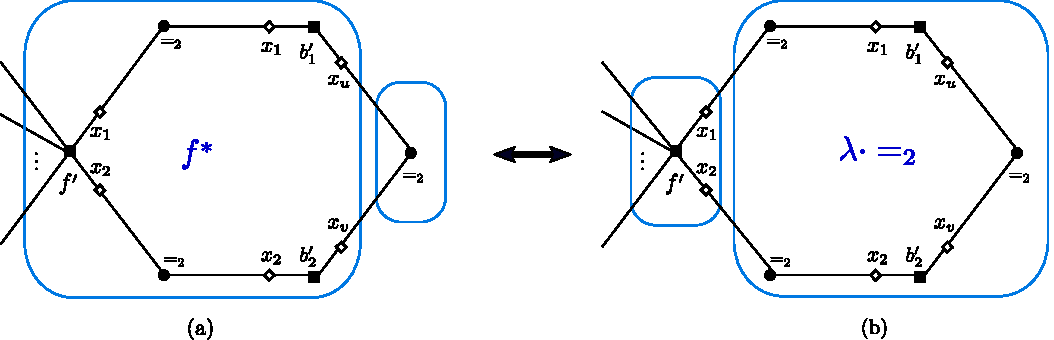
\includegraphics[height=4.8cm]{f_ast-f.pdf}
    \caption{\cite{realholant} Gadget constructions of ${\partial}_{12}{{f^\ast}}$  and ${\partial}_{12}{{f'}}$}
    \label{fig:f^ast-f'}
\end{figure}

Then, we show that  ${\partial}_{st}{f^{\ast}}\in {\mathcal{E}}^{\otimes}$ for all pairs of indices $\{s, t\}$ disjoint with $\{1, 2, i, j\}$ and $\{s, t\} \neq \{u, v\}$ where $u$ and $v$ are named in (\ref{form_ij}). 
Clearly, ${\partial}_{st}{f^{\ast}}\not\equiv 0$ since ${\partial}_{(st)(12)}{f^{\ast}}\in{\mathcal{E}}^{\otimes}$.
 We first show that in the UPF of ${\partial}_{st}{f^{\ast}}$, $x_1$ and $x_2$ appear in two distinct nonzero binary signatures. 
 Otherwise, for a contradiction, suppose that there is a nonzero binary signature ${b^\ast}(x_1, x_2)$ such that ${b^\ast}(x_1, x_2)\mid {\partial}_{st}{f^{\ast}}$. 
 Then, ${b^\ast}(x_1, x_2)\mid{\partial}_{(ij)(st)}{f^{\ast}}={\partial}_{(st)(ij)}{f^{\ast}}\not\equiv 0$. 
 By the form (\ref{form_ij}) of ${\partial}_{ij}{f^{\ast}}$,  
 the only way that $x_1$ and $x_2$ can form a nonzero binary signature in ${\partial}_{(st)(ij)}{f^{\ast}}$ is that the merging gadget is actually merging $x_u$ and $x_v$. Thus, $\{s, t\}=\{u, v\}$. Contradiction. 
Therefore, for some $i'$ and $j'$, we have 
\begin{equation}\label{form_st}
{\partial}_{st}{f^{\ast}}={b^\ast_{st1}}(x_1, x_{i'})\otimes {b^\ast_{st2}}(x_2, x_{j'})\otimes{h_{st}},
%\in {\mathcal{E}}^{\otimes}.
\end{equation}
%Since ${\partial}_{(12)(st)}{f^{\ast}}\in {\mathcal{E}}^{\otimes}$, 
%all three signatures 
for some ${b^\ast_{st1}}(x_1, x_{i'}),  {b^\ast_{st2}}(x_2, x_{j'}), {h_{st}} \not \equiv 0$ since  ${\partial}_{st}{f^{\ast}}\not\equiv 0$.
  Since ${h_{st}} \mid {\partial}_{(12)(st)}{f^\ast}$ and ${\partial}_{(12)(st)}{f^\ast}\in 
    %{\int_2}
    {\mathcal{E}}^{\otimes}$, 
%and furthermore 
we have ${h_{st}} \in {\mathcal{E}}^{\otimes}$.
Also, by \cref{lem-binary-sim}, ${b^\ast_{st1}}  \sim \overline{b^\ast_{st2}}$.
For a contradiction,
suppose that ${\partial}_{st}{f^{\ast}}\notin {\mathcal{E}}^{\otimes}$, then  ${b^\ast_{st1}}(x_1, x_{i'}) 
%\sim {b^\ast_{st2}}(x_2, x_\ell)  
\not\sim (=_2)$,
and ${b^\ast_{st2}}(x_2, x_{j'})  
\not\sim (=_2)$.
Consider the signature ${\partial}_{(st)(ij)}{f^{\ast}}$. 
Since $\{s, t\}\neq \{u, v\}$,  by the form (\ref{form_ij}) of ${\partial}_{ij}{f^{\ast}}$, 
$x_1$ and $x_2$ appear in two binary signatures in the UPF of ${\partial}_{(st)(ij)}{f^{\ast}}.$
Remember that ${\partial}_{(st)(ij)}{f^{\ast}}={\partial}_{(ij)(st)}{f^{\ast}}$.
By the form (\ref{form_st}) of ${\partial}_{st}{f^{\ast}}$, 
if
$\{i', j'\}= \{i, j\}$, 
then, after merging $x_i$ and $x_j$ of ${\partial}_{st}{f^{\ast}}$, $x_1$ and $x_2$ will form a new binary  signature in ${\partial}_{(ij)(st)}{f^{\ast}}$. Contradiction.
Thus, $\{i', j'\}\neq \{i, j\}$.
Then, when merging $x_i$ and $x_j$ of ${\partial}_{st}{f^{\ast}}$,
among ${b^\ast_{st1}}(x_1, x_{i'})$ and ${b^\ast_{st2}}(x_2, x_{j'})$, at least one binary signature is untouched. 
Thus, ${\partial}_{(ij)(st)}{f^{\ast}}$ has a factor that is not an associate of $=_2$. 
Contradicting ${\partial}_{(ij)(st)}{f^{\ast}}\in {\mathcal{E}}^{\otimes}$,
which is a consequence of (\ref{form_ij}).
Thus, ${\partial}_{st}{f^{\ast}}\in {\mathcal{E}}^{\otimes}$.

Then, we show that ${\partial}_{uv}{f^{\ast}} \in {\mathcal{E}}^{\otimes}$. 
Recall the form (\ref{form_ij}) of ${\partial}_{ij}{f^{\ast}}$. Clearly, $\{u, v\}$ is disjoint with $\{1, 2, i, j\}$.
Also, ${\partial}_{uv}{f^{\ast}}\not\equiv 0$ since ${\partial}_{(ij)(uv)}{f^{\ast}} \in {\mathcal{E}}^{\otimes}.$
Consider the UPF of ${\partial}_{uv}{f^{\ast}}$.
%Recall the form (\ref{form_ij}).
\begin{itemize}
    \item 
If $x_1$ and $x_2$ appear in one nonzero binary signature ${b^\ast_{uv}}(x_1, x_2)$, then $${\partial}_{uv}{f^{\ast}}={b^\ast_{uv}}(x_1, x_2)\otimes {g_{uv}} ~~~~\text{ for some } {g_{uv}} \not\equiv 0.$$
%\in {\mathcal{E}}^{\otimes}.$$
%Here ${b^\ast_{uv}}$
%is nonzero and $ {g_{uv}}\in {\mathcal{E}}^{\otimes}$,  because  we already have
%${\partial}_{12}{f^{\ast}}\in {\mathcal{E}}^{\otimes}$,
% and   
%${\partial}_{(12)(uv)}{f^{\ast}} \in 
%{\mathcal{E}}^{\otimes}$
%which is nonzero, 
% and
Then, we have
 ${g_{uv}} \sim
 {\partial}_{(12)(uv)}{f^{\ast}} \in 
{\mathcal{E}}^{\otimes}$ since ${\partial}_{12}{f^{\ast}}\in {\mathcal{E}}^{\otimes}$.
Also, since ${b^\ast_{uv}}(x_1, x_2)\mid {\partial}_{(ij)(uv)}{f^{\ast}}\in {\mathcal{E}}^{\otimes}$, we have ${b^\ast_{uv}}(x_1, x_2)\in {\mathcal{E}}^{\otimes}$. Hence, ${\partial}_{uv}{f^{\ast}}\in {\mathcal{E}}^{\otimes}$.
%we show $x_1$ and $x_2$ must appear in one single binary. 
\item If $x_1$ and $x_2$ appear in two distinct nonzero binary signatures ${b^\ast_{uv1}}(x_1, x_{i'})$ and ${b^\ast_{uv2}}(x_2, x_{j'})$, then
 $${\partial}_{uv}{f^{\ast}}={b^\ast_{uv1}}(x_1, x_{i'})\otimes {b^\ast_{uv2}}(x_2, x_{j'})\otimes{h_{uv}} ~~~~\text{ for some } {h_{uv}}\not\equiv 0.$$
 %\in {\mathcal{E}}^{\otimes}.$$ 
 
% In view of (\ref{eqn:lm5-partial12-f}), by considering
% ${\partial}_{(uv)(12)}{f^{\ast}}$
% we see that both binary signatures ${b^\ast_{uv1}}(x_1, x_{i'}) \not \equiv 0$,  ${b^\ast_{uv2}}(x_2, x_{j'}) \not \equiv 0$
% and 
Then, we have $ {h_{uv}} \in {\mathcal{E}}^{\otimes}$ since ${\partial}_{(12)(uv)}{f^{\ast}} \in 
{\mathcal{E}}^{\otimes}$. 
By the form (\ref{form_ij}) of ${\partial}_{ij}{f^{\ast}}$, 
after merging variables $x_u$ and $x_v$ of  ${\partial}_{ij}{f^{\ast}}$,
variables $x_1$ and $x_2$ form a binary $=_2$ in ${\partial}_{(uv)(ij)}{f^{\ast}}={\partial}_{(ij)(uv)}{f^{\ast}}$. 
On the other hand,
by the form of ${\partial}_{uv}{f^{\ast}}$, the only way that $x_1$ and $x_2$  form a binary after merging two variables in ${\partial}_{uv}{f^{\ast}}$ is to merge  $x_{i'}$ and $x_{j'}$. 
Thus, we have $\{i', j'\}=\{i, j\}$. Since ${f^{\ast}}$ has arity $2n \geqslant 8$, we can find another pair of indices $\{s, t\}$ disjoint with $\{1, 2, i, j, u, v\}$. 
When merging variables $x_s$ and $x_t$ in ${\partial}_{uv}{f^{\ast}}$, 
binary signatures ${b^\ast_{uv1}}(x_1, x_{i'})$ and ${b^\ast_{uv2}}(x_2, x_{j'})$ are untouched. 
Thus, we have ${b^\ast_{uv1}}(x_1, x_{i'})\otimes {b^\ast_{uv2}}(x_2, x_{j'})\mid {\partial}_{(st)(uv)}{f^{\ast}}$.
As showed above, we have ${\partial}_{st}{f^{\ast}}\in {\mathcal{E}}^{\otimes}$ and then  ${\partial}_{(st)(uv)}{f^{\ast}}\in {\mathcal{E}}^{\otimes}$.
Thus, ${b^\ast_{uv1}}(x_1, x_{i'})\otimes {b^\ast_{uv2}}(x_2, x_{j'})\in {\mathcal{E}}^{\otimes}$ and then ${\partial}_{uv}{f^{\ast}}\in {\mathcal{E}}^{\otimes}$.
\end{itemize}

So far, we have shown that ${\partial}_{12}{f^{\ast}}\in {\mathcal{E}}^{\otimes}$, ${\partial}_{ij}{f^{\ast}}\in {\mathcal{E}}^{\otimes}$ and ${\partial}_{st}{f^{\ast}}\in {\mathcal{E}}^{\otimes}$ for all $\{s, t\}$ disjoint with $\{1, 2, i, j\}$.
If we can further show that ${\partial}_{ik}{f^{\ast}}\in {\mathcal{E}}^{\otimes}$ for all $k\neq 1, 2, i, j$, and then symmetrically ${\partial}_{jk}{f^{\ast}}\in {\mathcal{E}}^{\otimes}$ for all $k\neq 1, 2, i, j$, then 
%Now, we want to show that,
${\partial}_{st}{f^{\ast}}\in {\mathcal{E}}^{\otimes}$ for all $\{s, t\}$  disjoint with $\{1, 2\}$.
Thus, by our \cref{claim: strong equality property},  ${f^\ast}\in {\int}\mathcal{E}^{\otimes}$. This will finish the proof of Case 2.

%Given what we have shown above, we only need to show that ${\partial}_{ik}{f^{\ast}}\in {\mathcal{E}}^{\otimes}$ for all $k\neq 1, 2, i, j$. 
%Then, by symmetry, we also have ${\partial}_{jk}{f^{\ast}}\in {\mathcal{E}}^{\otimes}$ for all $k\neq 1, 2, i, j$. 
%Thus, ${\partial}_{st}{f^{\ast}}\in {\mathcal{E}}^{\otimes}$ for all $\{s, t\}$ that is disjoint with or equal to $\{1, 2\}$. 
%Then, we may switch the roles
%of (\ref{eqn:lm5-partial12-f}) and
%(\ref{form_ij})
%and switch the roles 
%of the pairs $\{1,2\}$ 
%and $\{i, j\}$.
%This will let us prove
%that
%as showed in Case 1, we have
%${\partial}_{1k}{f^\ast}\in {\mathcal{E}}^{\otimes}$ and ${\partial}_{2k}{f^\ast}\in {\mathcal{E}}^{\otimes}$ for all $3 \leqslant k \leqslant 2n$.
%$k \not = 1, 2, i, j$.
%Combining these results, we finally get
%$3 \leqslant k \leqslant 2n$. 
%Thus,
%${f^{\ast}}\in {\int}{\mathcal{E}}^{\otimes}$.

Now we prove ${\partial}_{ik}{f^{\ast}}\in {\mathcal{E}}^{\otimes}$ for all $k\neq 1, 2, i, j$. 
%Then, by symmetry, we also have ${\partial}_{jk}{f^{\ast}}\in {\mathcal{E}}^{\otimes}$ for all $k\neq 1, 2, i, j$. 
%Consider ${\partial}_{ik}{f^{\ast}}$ for any $k\neq 1, 2, i, j$. 
Since ${\partial}_{(ik)(12)}{f^{\ast}}\in \mathcal{E}^{\otimes}$,
we have  ${\partial}_{ik}{f^{\ast}}\not\equiv 0$. 
So we can consider the UPF
of ${\partial}_{ik}{f^{\ast}}$. 
\begin{itemize}
    \item 
If $x_1$ and $x_2$ appear in one nonzero binary signature, then  $${\partial}_{ik}{f^{\ast}}={b^\ast_{ik}}(x_1, x_2)\otimes {g_{ik}} ~~~~\text{ for some } {g_{ik}}\in \mathcal{E}^{\otimes}.$$ 
Here, ${g_{ik}}\in \mathcal{E}^{\otimes}$
since ${\partial}_{(ik)(12)}{f^{\ast}}
\in \mathcal{E}^{\otimes}$.
Since ${f^\ast}$ has arity $2n \geqslant 8$,
we can pick a pair of indices $\{s, t\}$ disjoint with $\{1, 2, i, j, k\}$, and merge variables $x_s$ and $x_t$ of ${\partial}_{ik}{f^{\ast}}$.
Then, ${b^\ast_{ik}}(x_1, x_2)\mid {\partial}_{(st)(ik)}{f^{\ast}}.$
Since ${\partial}_{st}{f^{\ast}}\in \mathcal{E}^{\otimes}$,
${\partial}_{(st)(ik)}{f^{\ast}}={\partial}_{(ik)(st)}{f^{\ast}}\in {\mathcal{E}}^{\otimes}$. Thus, ${b^\ast_{ik}}(x_1, x_2) \in {\mathcal{E}}^{\otimes}$ and then ${\partial}_{ik}{f^{\ast}}\in {\mathcal{E}}^{\otimes}$.
\item    If $x_1$ and $x_2$ appear in two nonzero distinct binary signatures,
then $${\partial}_{ik}{f^{\ast}}={b^\ast_{ik1}}(x_1, x_p)\otimes {b^\ast_{ik2}}(x_2, x_q)\otimes{h_{ik}} ~~~~\text{ for some } {h_{ik}} \in \mathcal{E}^{\otimes}.$$
Again, here ${h_{ik}} \in \mathcal{E}^{\otimes}$
since ${\partial}_{(ik)(12)}{f^{\ast}}
\in \mathcal{E}^{\otimes}$.
By connecting variables $x_1$ and $x_2$ of ${\partial}_{ik}{f^{\ast}}$, $x_p$ and $x_q$ will form a binary $=_2$ up to a nonzero scalar
(this binary signature is $=_2$
because we know that
 ${\partial}_{(ik)(12)}{f^{\ast}}\in \mathcal{E}^{\otimes}$).
By \cref{lem-binary-sim}, 
as the type of binary signatures,
${{b^\ast_{ik1}}} \sim \overline{b^\ast_{ik2}}.$
%${{b^\ast_{ik1}}}(x_1, x_p) \sim {b^\ast_{ik2}}(x_2, x_q).$
Between $x_p$ and $x_q$, at least one of them is not $x_j$; suppose that it is $x_p$. 
We pick a variable $x_r$ in the scope of ${h_{ik}}$ that is also not $x_j$ (such a  variable $x_r$  exists as $2n \geqslant 8$). Then, by merging $x_p$ and $x_r$ of ${\partial}_{ik}{f^{\ast}}$, 
the binary signature ${b^\ast_{ik2}}(x_2, x_q)$ is untouched. 
Since $\{p, r\}$ is disjoint with $\{1, 2, i, j\}$, we have ${b^\ast_{ik2}}(x_2, x_q)\mid {\partial}_{(ik)(pr)}{f^{\ast}}\in {\mathcal{E}}^{\otimes}$. Thus, we have ${b^\ast_{ik2}}(x_2, x_q)
% JYC edited out this   {f^{\ast}}
\in {\mathcal{E}}^{\otimes}$ and so does
${{b^\ast_{ik1}}}(x_1, x_p)$. 
Thus, ${\partial}_{ik}{f^{\ast}}\in {\mathcal{E}}^{\otimes}$.
    \end{itemize}
%We show ${\partial}_{st}{f^{\ast}}\in $
   
    
   % Thus, we know connecting $x_1$ of ${b'_1}$ with $x_2$ of ${b'_2}$ gives $\neq_2$. This implies that ${b'_1}$ and ${b'_2}$ are both in ${\mathcal{U}^{\otimes}_{1}}$ or ${\mathcal{U}^{\otimes}_{0}}$. 
%Thus, we have
As remarked earlier,  by symmetry, we also have ${\partial}_{jk}{f^{\ast}}\in {\mathcal{E}}^{\otimes}$ for all $k\neq 1, 2, i, j$. Thus, we are done with Case 2.
%can realize a signature ${f^\ast}$ of arity $2n$ from ${f'}$ such that
%${f^\ast}\in {\int}{\mathcal{E}}^{\otimes}$. 

Thus, an irreducible signature ${f^\ast}\in \int\mathcal{E}^{\otimes}$ of arity $2n$ is realized from $ f$.
\end{proof}

We next determine the exact form of an arity-$8$ signature with the strong equality property. 
By \cref{lm: unitary wire normalization}, we may assume that $\mathcal{F}$ contains an arity $8$ signature $h$ satisfying the strong equality property.
Otherwise, the induction is completed by the first two items in \cref{lm: unitary wire normalization}.

\begin{definition}\label{def: f8 matching}
    Let $h\in \mathcal{F}$ be an arity 8 signature satisfying the strong equality property.
    By \cref{def: Strong equality property}, for any pair of distinct indices $e=\{i,j\}$, $$\partial_{e}h=\partial_{ij}h=\lambda_{ij}\cdot (=_2)(x_{i_1},x_{j_1})\cdot(=_2)(x_{i_2},x_{j_2})\cdot (=_2)(x_{i_3},x_{j_3}), \quad \lambda_{ij}\in \C^\times,$$
    and $\{i,j\}\cup \{i_1,j_1\}\cup\{i_2,j_2\}\cup\{i_3,j_3\}=\{1,2,\ldots, 8\}.$
    We define $M_e=\{\{i_1,j_1\},\{i_2,j_2\},\{i_3,j_3\}\}$ and $F_e=\{i,j\}\cup M_e.$
    For two pairs of distinct indices $e_1=\{i,j\}$ and $e_2=\{k,\ell\}$, define $e_1\sim e_2$ if $e_1\in F_{e_2}$.
\end{definition}

\begin{lemma}\label{lm: f8 matching same norm}
    The $\lambda_{ij}$ in \cref{def: f8 matching} have the same norm for every pair of distinct indices $\{i,j\}$, otherwise $\Holant(\mathcal{F})$ is \#P-hard.
\end{lemma}
\begin{proof}
    We may assume $h$ is irreducible and satisfies {\sc 2nd-Orth}, otherwise we obtain $\Holant(\mathcal{F})$ is \#P-hard.
    By \cref{lm: 2nd-orth contraction nonzero}, $|\partial_{ij}f|^2=\lambda\cdot |(=_2)|^2=2\lambda$ for every pair of distinct indices $\{i,j\}$, where $\lambda=|f_{ij}^{00}|^2=|f_{ij}^{01}|^2=|f_{ij}^{10}|^2=|f_{ij}^{11}|^2>0$.
    On the other hand, $|\partial_{ij}f|^2=|\lambda_{ij}|^2\cdot \prod_{k=1}^3|(=_2)(x_{i_k},x_{j_k})|^2=8|\lambda_{ij}|^2.$
    Therefore, $|\lambda_{ij}|$ are all the same.
\end{proof}

\begin{lemma}\label{lm: f8 matching equivalence}
    The relation ``$\sim$'' in \cref{def: f8 matching} is an equivalence relation, otherwise $\Holant(\mathcal{F})$ is \#P-hard.
\end{lemma}
\begin{proof}
    First $M_e$ and $F_e$ are well defined for any pair of indices $e=\{i,j\}$, by the UPF of $\partial_eh.$
    Clearly $e\in F_e$, so $\sim$ is self-inversive.
    %Next we show $\sim$ is reflexive and transitive.
    
    Now suppose $d=\{k,\ell\}$ and $e=\{i,j\}$ are two pairs of distinct indices such that $d\neq e$ and $d\sim e$. 
    Then $d\in M_e$ and $d\cap e=\emptyset.$
    Suppose $M_e=\{\{k,\ell\},\{s,t\},\{u,v\}\}.$
    Then
    \begin{equation}\label{eq: contract h using e}
        \partial_{ij}h=\lambda_{ij}\cdot (=_2)(x_{k},x_{\ell})\cdot (=_2)(x_{s},x_{t})\cdot (=_2)(x_{u},x_{v}).
    \end{equation}
    Suppose $M_d=\{\{i_1,j_1\},\{i_2,j_2\},\{i_3,j_3\}\}$, then 
    \begin{equation}\label{eq: contract h using d}
        \partial_{k\ell}h=\lambda_{k\ell}\cdot (=_2)(x_{i_1},x_{j_1})\cdot (=_2)(x_{i_2},x_{j_2})\cdot (=_2)(x_{i_3},x_{j_3}).
    \end{equation}
    Consider $\partial_{(k\ell)(ij)}h=\partial_{(ij)(k\ell)}h$.
    By \eqref{eq: contract h using e}, we have 
    \begin{equation}\label{eq: contracting h by e then d}
        \partial_{(k\ell)(ij)}h=2\lambda_{ij}\cdot (=_2)(x_{s},x_{t})\cdot (=_2)(x_{u},x_{v}).
    \end{equation} 
    Suppose for a contradiction that $e\notin M_d$.
    Then $x_i$ and $x_j$ appear in two distinct binary factors in \eqref{eq: contract h using d}. 
    Without loss of generality, $i=i_1$ and $j=j_2$.
    Merging $x_i$ and $x_j$ results in 
    \begin{equation}\label{eq: contracting h using d then e}
        \partial_{(ij)(k\ell)}h=\lambda_{k\ell}\cdot (=_2)(x_{j_1},x_{i_2})\cdot (=_2)(x_{i_3},x_{j_3}).
    \end{equation}
    Compare \eqref{eq: contracting h by e then d} and \eqref{eq: contracting h using d then e}, we have $2\lambda_{ij}=\lambda_{k\ell}.$
    However, by \cref{lm: f8 matching same norm}, $|\lambda_{ij}|=|\lambda_{k\ell}|>0$, contradiction.
    Therefore, $e\in M_d$.
    Without loss of generality, $i=i_1$ and $j=j_1$.
    Then 
    \begin{equation}\label{eq: contracting h using d then e 2}
        \partial_{(ij)(k\ell)}h=2\lambda_{k\ell}\cdot (=_2)(x_{i_2},x_{j_2})\cdot (=_2)(x_{i_3},x_{j_3}).
    \end{equation}
    Compare \eqref{eq: contracting h by e then d} and \eqref{eq: contracting h using d then e 2}, we have $\lambda_{ij}=\lambda_{k\ell}.$
    Thus, $\sim$ is reflective.
    Moreover, if $d\in M_e$, then $\lambda_d=\lambda_e.$

    Finally we show transitivity.
    Suppose $c=\{s,t\},d=\{k,\ell\},e=\{i,j\}$, and $c\sim d,\,d\sim e$.
    If any two of them are equal, then trivially $c\sim e.$
    Now assume $c,d,e$ are mutually distinct.
    We have $c\in M_d$ and $d\in M_e$.
    So $\{s,t\}\cap\{k,\ell\}=\emptyset$ and $\{k,\ell\} \cap \{i,j\}=\emptyset.$
    Suppose 
    \begin{equation}\label{eq: transitivity partial e h}
        \partial_{ij}h=\lambda_{ij}\cdot (=_2)(x_k,x_{\ell})\cdot (=_2)\cdot (=_2).
    \end{equation}
    By reflectivity, $e\in M_d$.
    Also $c\in M_d$ and $c\neq e$.
    So $\{k,\ell\}\cap\{i,j\}=\emptyset$ and
    \begin{equation}\label{eq: transitivity partial d h}
        \partial_{k\ell}h=\lambda_{k\ell}\cdot (=_2)(x_i,x_{j})\cdot (=_2)(x_s,x_t)\cdot (=_2).
    \end{equation}
    Now consider $\partial_{(st)(ij)(k\ell)}h=\partial_{(st)(k\ell)(ij)}h$.
    By \eqref{eq: transitivity partial d h}, $\partial_{(st)(ij)(k\ell)}h=4\lambda_{k\ell}\cdot(=_2)$.
    Suppose for a contradiction that $c\notin M_e$.
    Then $s$ and $t$ appear in the second and third binary factors respectively in \eqref{eq: transitivity partial e h}.
    So $\partial_{(st)(k\ell)(ij)}h=2\lambda_{ij}\cdot(=_2)$.
    We obtain $4\lambda_{k\ell}=2\lambda_{ij}>0$, contradiction.
    So $c\in M_e$ and thus $c\sim e$.
    
    We have proved $\sim$ is self-inversive, reflexive and transitive. 
    So it is an equivalence relation. 
\end{proof}

\begin{lemma}\label{lm: f8 same coe}
    The $\lambda_{ij}$ in \cref{def: f8 matching} are all the same, otherwise $\Holant(\mathcal{F})$ is \#P-hard.
\end{lemma}
\begin{proof}
    In the proof of \cref{lm: f8 matching equivalence}, we have proved $\lambda_{ij}$ are all the same for $\{i,j\}$ in the same equivalent class of $\sim.$
    We only need to show $\lambda_{ij}=\lambda_{k\ell}$ for $\{i,j\}\not \sim \{k,\ell\}.$
    Let $e=\{i,j\},\,d=\{k,\ell\}.$
    We have $\partial_{ij}h=\lambda_{ij}\cdot (=_2)^{\otimes 3}$
    and $\partial_{k\ell}h=\lambda_{k\ell}\cdot (=_2)^{\otimes 3}$.
    Since $\{i,j\}\not \sim\{k,\ell\}$, we know $d\notin M_e$ and $e\notin M_d.$
    So $x_k$ and $x_\ell$ appear in distinct binary factors of $\partial_{ij}h$.
    Then $\partial_{(k\ell)(ij)}h=\lambda_{ij}\cdot (=_2)^{\otimes 2}.$
    Similarly, $x_i$ and $x_j$ appear in distinct binary factors of $\partial_{k\ell}h$, and $\partial_{(ij)(k\ell)}h=\lambda_{k\ell}\cdot (=_2)^{\otimes 2}.$
    By $\partial_{(k\ell)(ij)}h=\partial_{(ij)(k\ell)}h$, we have $\lambda_{ij}=\lambda_{k\ell}$.
\end{proof}

An equivalent class of $\sim$ in \cref{def: f8 matching} can be viewed as a perfect matching of the complete graph $K_8$ with vertices labeled by $\{1,2,\ldots, 8\}.$
Since $K_8$ has 28 edges, and every equivalent class has size $4$, there are 7 equivalent classes in total.
They are 7 perfect matchings, or a 1-factorization of $K_8$.

\begin{lemma}
\label{lm: f8 one factorization}
%The equivalent classes $F_e$ form a $1$-factorization of $K_8$.
After identifying the vertices of $K_8$ with the points of
$\mathbb F_2^3$, the seven perfect matchings determined by the equivalent classes of $\sim$ are
\begin{equation}
    F_e=\bigl\{\{z,z+v_e\}\mid z\in\mathbb F_2^3\bigr\}, \qquad v_e\in\mathbb F_2^3\setminus\{0\}.
 \label{eq: translation matchings}
\end{equation}
\end{lemma}

\begin{proof}
Let $\mathcal{PM}$ be the 7 perfect matchings determined by the equivalent classes of $\sim$.
The union of two perfect matchings in $\mathcal{PM}$ is either one $8$-cycle or two $4$-cycles.  
The first case is impossible.  Indeed, label an alternating $8$-cycle so that the two perfect matchings are
\[
 F_1=\{\{1,2\},\{3,4\},\{5,6\},\{7,8\}\},\qquad
 F_2=\{\{2,3\},\{4,5\},\{6,7\},\{8,1\}\}.
\]
Merging first $x_1,x_2$ and then $x_4,x_5$ leaves the residual matching
$\{\{3,6\},\{7,8\}\}$.
By commutativity, it is equivalent to first merge $x_4,x_5$ and then $x_1,x_2$, leaving $\{\{3,8\}, \{6,7\}\}$.  
This contradicts the UPF of $\partial_{(12)(34)}h$.
Thus every two perfect matchings form two $4$-cycles.


For every perfect matching $F\in\mathcal{PM}$, we identify $F$ with a map $m_F:V(K_8)\to V(K_8)$, $u\mapsto v$ if $\{u,v\}\in F.$
So $m_F$ is an involution map, i.e., $m_F^{(2)}(u)=m_F(m_F(u))=u,\,\forall u\in [8].$
Let $G=\{m_F\mid F\in \mathcal{PM}\}\cup \{\mathrm{id}\}$.
Consider two perfect matchings $F_1,F_2\in \mathcal{PM}$.
Since $F_1\cup F_2$ form two 4-cycles of $K_8$, we have $m_{F_1}m_{F_2}=m_{F_2}m_{F_1}$.
Now fix one vertex $z_0\in V(K_8)$.
Given two maps $m_1,m_2\in G$, let $m_3$ be the unique member in $G$ satisfying $m_3(z_0)=m_1m_2(z_0)$.
This $m_3$ exists, because if $m_1=m_2$ then $m_3=\mathrm{id}$, otherwise it is the map determined by the matching containing the edge $\{z_0,m_1m_2(z_0)\}.$
For every $m\in G$, commutativity gives $m_3(m(z_0))=m(m_3(z_0))=m(m_1m_2(z_0))=m_1m_2(m(z_0))$.  
The eight points $\{m(z_0)\mid m\in G\}$ exhaust the vertex set, so $m_3=m_1m_2$.  
Thus, $G$ is an abelian group of
order eight, and every non-zero element in $G$ has order $2$.
Hence $G\cong \mathbb F_2^3$. 
Now we identify the vertex $m(z_0)\in V(K_8)$ with $m\in G\cong \mathbb F_2^3,\,\forall m\in G.$
Then the seven non-zero elements in $G$ are exactly \eqref{eq: translation matchings}.
\end{proof}

In the following, we give an interpretation of the signature $f_8$ through the lens of the Reed-Muller code $RM(1,3).$
Let
\begin{equation}
 C=RM(1,3)
 =\left\{(a_0+a\cdot z)_{z\in\mathbb F_2^3}\mid 
 a_0\in\mathbb F_2,\ a\in\mathbb F_2^3\right\}.
 \label{eq: RM code definition}
\end{equation}
The coordinates are ordered as
$000,001,010,011,100,101,110,111$.  Thus $C$ is the self-dual
$[8,4,4]$ first order Reed-Muller code, with codewords
\begin{align*}
&00000000,00001111,00110011,00111100,01010101,01011010,\notag\\
&01100110,01101001,10010110,10011001,10100101,10101010,\notag\\
&11000011,11001100,11110000,11111111.
\end{align*}
Therefore, $f_8=\chi_C.$

\begin{lemma}\label{lm: f8 indistinguishble}
    Let $h\in \mathcal{F}$ be an arity $8$ signature satisfying the strong equality property.
    Then there exists $\lambda\in \mathbb C^\times$ such that $\partial_{ij}h= \lambda\cdot\partial_{ij}f_8$ for every pair of distinct indices $\{i,j\},$ otherwise $\Holant(\mathcal{F})$ is \#P-hard.
\end{lemma}
\begin{proof}
    By \cref{lm: f8 same coe}, unless $\Holant(\mathcal{F})$ is \#P-hard, there exists $\lambda\in \mathbb C^\times$ such that 
    \begin{equation*}
        \partial_{e}h=\lambda\cdot\bigotimes_{d\in M_e}(=_2)_d
    \end{equation*}
    for every pair of indices $e=\{i,j\}$, where $(=_2)_d$ is the binary $=_2$ on the two variables corresponding to the two indices in $d.$
    By \cref{lm: f8 one factorization}, we may label $\{1,2,\ldots, 8\}$ by elements in $\mathbb F_2^3$, such that $F_e=\{\{z,z+v_e\}\mid z\in \mathbb{F}_2^3\}$ for some $v_e\in \mathbb F_2^3\setminus\{0\}.$
    Since $e\in F_e$, there exists some $z_0\in \mathbb F_2^3$ such that $e=\{z_0,z_0+v_e\}.$
    Suppose $M_e=\{\{z_1,z_1+v_e\},\{z_2,z_2+v_e\},\{z_3,z_3+v_e\}\}$ for some $z_1,z_2,z_3\in \mathbb F_2^3.$
    Then 
    \begin{equation}\label{eq: f8 indistinguishble partial e h}
        \partial_{e}h=\lambda\cdot\bigotimes_{i=1}^3(=_2)(x_{z_i},x_{z_i+v_e}).
    \end{equation}
    Now consider $\partial_{e}f_8$.
    Since $e=\{z_0,z_0+v_e\}$, merging $x_{z_0}$ and $x_{z_0+v_e}$ requires $x_{z_0}=x_{z_0+v_e}.$
    By the definition of $C=RM(1,3)$ and $f_8=\chi_C$, the $y$-th coordinate of the codeword indexed by $(a_0,a)$ is $x_y=a_0+a\cdot y.$
    So $x_{z_0}=x_{z_0+v_e}\iff a_0+a\cdot z_0=a_0+a\cdot (z_0+v_e)\iff a\cdot v_e=0.$
    Once $a\cdot v_e=0$, we have $x_{y+v_e}=a_0+a\cdot (y+v_e)=a_0+a\cdot y=x_y$, for every $y\in \mathbb F_2^3.$
    Therefore, $x_{z_i}=x_{z_i+v_e}$ in $\partial_{e}f_8$ for $i=1,2,3.$
    Direct computation shows that merging any two variables of $f_8$, it becomes a tensor product of three binary equalities \cite{realholant}.
    So
    \begin{equation}\label{eq: f8 indistinguishble partial e f8}
        \partial_{e}f_8=\bigotimes_{i=1}^3(=_2)(x_{z_i},x_{z_i+v_e}).
    \end{equation}
    Comparing \eqref{eq: f8 indistinguishble partial e h} and \eqref{eq: f8 indistinguishble partial e f8} gives $ \partial_{ij}h=\lambda\cdot\partial_{ij}f_8$, for every pair of indices $\{i,j\}$.
\end{proof}

\begin{lemma}
\label{lm: f8 normalized equations}
Let $h\in \mathcal{F}$ be an arity 8 signature satisfying the strong equality property. 
After normalizing $h$,
unless $\Holant(\mathcal{F})$ is \#P-hard,
there exists
$\alpha,\beta\in\mathbb C$ such that
\begin{equation}
 h= f_8+\alpha u_+^{\otimes8}+\beta u_-^{\otimes8}.
 \label{eq: f8 kernel family}
\end{equation}
where $u_+=[1, \mathfrak i], u_-=[1, -\mathfrak i]$ are unary signatures.
Moreover, $h$ satisfies {\sc 2nd-Orth} if and only if
\begin{equation}
 \operatorname{Re}(\alpha)+8|\alpha|^2=0,
 \qquad
 \operatorname{Re}(\beta)+8|\beta|^2=0.
 \label{eq: f8 second orth circles}
\end{equation}
\end{lemma}

\begin{proof}
By \cref{lm: f8 indistinguishble}, there exists $\lambda\in \mathbb C^\times$ such that $\partial_{ij}h=\lambda\cdot \partial_{ij}f_8$ for every pair of distinct indices $\{i,j\}.$
We normalize $h$ by $\lambda$, and with a slight abuse of notation, still use $h$ to denote the normalized signature.
Let $h'=h-f_8$.
Then $\partial_{ij}h'=0$ for every pair of distinct indices $\{i,j\}.$
Notice that $\{u_+,u_{-}\}$ form a basis for $\C^2$.
So $\{u_{\epsilon_1}\otimes u_{\epsilon_2}\otimes\ldots \otimes u_{\epsilon_8}\mid \epsilon_1,\epsilon_2,\ldots,\epsilon_8\in\{+,-\}\}$ form a basis for $(\C^2)^8$.
The arity $8$ signature $h'$ can be viewed as a tensor in $(\C^2)^8.$
We expand $h'$ interms of this basis, and obtain
\begin{equation}\label{eq: expansion of h'}
    h'=\sum_{\epsilon_1,\ldots, \epsilon_8\in\{+,-\}}c'_{\epsilon_1,\ldots,\epsilon_8}u_{\epsilon_1}\otimes\ldots\otimes u_{\epsilon_8}=\sum_{S\subseteq[8]}c_S \bigotimes_{j\in S}u_+ \bigotimes_{j\notin S}u_{-},
\end{equation}
where $c_S=c'_{\epsilon_1,\ldots,\epsilon_8}$ if $S=\{i\in[8]\mid \epsilon_i=+\}.$
We note that
\begin{equation}
 u_+u_+^{\mathtt T}=u_-u_-^{\mathtt T}=0,\qquad
 u_+u_-^{\mathtt T}=u_-u_+^{\mathtt T}=2.
 \label{eq: isotropic unary basis}
\end{equation}
Now consider $\partial_{ij}h'.$
By \eqref{eq: isotropic unary basis}, every term in \eqref{eq: expansion of h'} with $\epsilon_i=\epsilon_j$ will vanish in $\partial_{ij}h'$, because merging $x_i$ and $x_j$ results in a factor $u_{\epsilon_i}u_{\epsilon_j}^{\tt T}.$
\begin{claim}\label{claim: Johnson graph}
    For every subset $T\subseteq[8]\setminus\{i,j\}$, the coefficients in \eqref{eq: expansion of h'} satisfy $c_{T\cup\{i\}}+c_{T\cup\{j\}}=0.$
\end{claim}
\begin{claimproof}{\cref{claim: Johnson graph}}
    Let $v_T:=\bigotimes_{j\in T} u_+\bigotimes_{j\in [8]\setminus\{i,j\}\setminus T}u_-.$
    After merging $x_i$ and $x_j$, $v_T$ is a term in the expansion of $\partial_{ij}h'$.
    We consider the coefficient of $v_T$ in $\partial_{ij}h'.$
    If a term in \eqref{eq: expansion of h'} survives in $\partial_{ij}h'$, then $\epsilon_i\neq\epsilon_j.$
    There are two possibilities, $(\epsilon_i,\epsilon_j)=(+,-)$ or $(\epsilon_i,\epsilon_j)=(-,+).$
    In the first case, the contribution for the coefficient of $v_T$ in $\partial_{ij}h'$ is $2c_{T\cup \{i\}}.$
    In the latter case, the contribution is $2c_{T\cup \{j\}}.$
    Hence the coefficient of $v_T$ in $\partial_{ij}h'$ is $2c_{T\cup \{i\}}+2c_{T\cup \{j\}}.$
    Since $\partial_{ij}h'=0$, and the terms $v_T$ are linearly independent, we have $c_{T\cup\{i\}}+c_{T\cup \{j\}}=0$, for every $T\subseteq[8]\setminus \{i,j\}.$
\end{claimproof}

\begin{claim}\label{claim: coe is 0 in expansion of h}
    In \eqref{eq: expansion of h'}, the coefficients $c_S=0$ if $1\le |S|\le 7$.
\end{claim}
\begin{claimproof}{\cref{claim: coe is 0 in expansion of h}}
    Fix \(1\le t\le 7\), and look only at coefficients \(c_S\) in \eqref{eq: expansion of h'} with $|S|=t$.
    Consider the Johnson graph $J(8,t)$, where the vertices are $t$-element subsets of [8], and two vertices are adjacent when the intersection of the two vertices (subsets) contains $t-1$ elements.
    By \cref{claim: Johnson graph}, whenever two subsets $S_1$ and $S_2$ are adjacent in $J(8,t)$, their coefficients $c_{S_1}$ and $c_{S_2}$ are negatives.
    We claim every vertex in $J(8,t)$ is contained in a triangle.
    To see this, pick an arbitrary vertex (subset) $S$.
    If $1\le t\le 6$, there are distinct elements $p,q,r\in [8]$ such that $p\in S$ and $q,r\notin S$.
    Let $S_1=S\setminus\{p\}\cup \{q\}$ and $S_1=S\setminus\{p\}\cup \{r\}$. 
    Then $S,S_1,S_2$ form a triangle in $J(8,t)$.
    If $t=7$, then $J(8,7)$ is the complete graph $K_8$, so every vertex is in a triangle.
    Along the triangle, we have $c_S+c_{S_1}=0\,,c_{S_1}+c_{S_2}=0\,,c_{S_2}+c_{S}=0\,$.
    So $c_S=0$.
\end{claimproof}
By \cref{claim: coe is 0 in expansion of h}, the expansion \eqref{eq: expansion of h'} simplifies to $h'=c_{\emptyset}u_+^{\otimes 8}+c_{[8]}u_-^{\otimes 8}.$
Let $\alpha=c_{\emptyset}$ and $\beta=c_{[8]}$, we have $h= f_8+\alpha u_+^{\otimes8}+\beta u_-^{\otimes8}.$

It remains to impose {\sc 2nd-Orth}.  The affine group of
$\mathbb F_2^3$ is transitive on pairs of coordinates, so it suffices to
compute the Gram matrix for one pair.  Put
\[
 E_-=2\operatorname{Re}(\alpha-\beta)
       +16(|\alpha|^2-|\beta|^2),\qquad
 E_+=2\operatorname{Re}(\alpha+\beta)
       +16(|\alpha|^2+|\beta|^2).
\]
For the four slices ordered as $00,01,10,11$, direct substitution into
$M_{12}(h)M_{12}(h)^\dagger$ gives
\begin{equation}
 D I_4+4
 \begin{bmatrix}
 0&-\mathfrak iE_-&-\mathfrak iE_-&-E_+\\
 \mathfrak iE_-&0&E_+&-\mathfrak iE_-\\
 \mathfrak iE_-&E_+&0&-\mathfrak iE_-\\
 -E_+&\mathfrak iE_-&\mathfrak iE_-&0
 \end{bmatrix},
 \label{eq: f8 slice Gram matrix}
\end{equation}
where
$D=4+8\operatorname{Re}(\alpha+\beta)
  +64(|\alpha|^2+|\beta|^2)$.
The matrix in \eqref{eq: f8 slice Gram matrix} is scalar precisely when
$E_-=E_+=0$, and these two equations are equivalent to
\eqref{eq: f8 second orth circles}.  Pair transitivity proves sufficiency
for every coordinate pair.
\end{proof}

%The two circles in \eqref{eq: f8 second orth circles} still leave a two-real-parameter family.  A four-ary self-mating gadget removes the extra freedom by invoking the completed arity-$4$ case, \cref{lm: base case 2n=4}.

\begin{lemma}
\label{lm: f8 self mating}
Let $h$ satisfy \eqref{eq: f8 kernel family} and
\eqref{eq: f8 second orth circles}.  
Unless $\Holant(\mathcal{F})$ is
\#P-hard, there exists $\theta\in\mathbb R$ such that
\begin{equation}
 h=R_\theta^{\otimes8}f_8,\qquad
 R_\theta=
 \begin{bmatrix}
 \cos\theta&\sin\theta\\
 -\sin\theta&\cos\theta
 \end{bmatrix}.
 \label{eq: f8 real orbit}
\end{equation}
\end{lemma}

\begin{proof}
Take two copies of $h$, join six corresponding variables using $(=_2)$,
and leave the first two variables of each copy dangling.  
(Notice that this is a self-mating, not mating $h$ and $\overline{h}$.)
Let $g_4$ be the
resulting four-ary signature.  With row order $00,01,10,11$ on the two
variables from the first copy and the same column order on those from the
second copy, substitution of \eqref{eq: f8 kernel family} gives
\begin{equation}\label{eq: f8 self mating matrix}
     M_{12,34}(g_4)=
     \begin{bmatrix}
     4+t&0&0&-t\\
     0&4+t&t&0\\
     0&t&4+t&0\\
     -t&0&0&4+t
     \end{bmatrix},\qquad t=8(\alpha+\beta+16\alpha\beta).
\end{equation}


The signature $g_4$ is nonzero.  By \cref{lm: base case 2n=4},  $g_4\in\mathcal U^{\otimes}$ unless $\Holant(\mathcal{F})$ is \#P-hard. 
An arity $4$ signature in $\mathcal U^{\otimes}$ has rank one in the $2|2$ flattening associated with its binary factorization. 
There are three possibilities, $M_{12,34}(g_4)$, or $M_{13,23}(g_4)$, or $M_{14,23}(g_4)$ has rank $1.$  
If $M_{12,34}(g_4)$ has rank 1, by evaluating all 2 by 2 minors in \eqref{eq: f8 self mating matrix}, we have $(4+t)^2=t^2=0$, which is impossible.
In the second case, evaluate all 2 by 2 minors in
    \[M_{13,24}(g_4)
    =
    \begin{bmatrix}
    4+t&0&0&4+t\\
    0&-t&t&0\\
    0&t&-t&0\\
    4+t&0&0&4+t
    \end{bmatrix},\]
we have $t(4+t)=0$.  
In the third case, 
    \[M_{14,23}(g_4)=
    \begin{bmatrix}
    4+t&0&0&t\\
    0&-t&4+t&0\\
    0&4+t&-t&0\\
    t&0&0&4+t
    \end{bmatrix}.\]
gives $(4+t)t=0$ and $t^2=(4+t)^2$, again impossible.

Thus, only second case is possible.
And $t=0$ or $t=-4.$
Now define
\(
 z=1+16\alpha,\, w=1+16\beta.
\)
The equations in \eqref{eq: f8 second orth circles} gives 
\(
|z|^2
=|1+16\alpha|^2
=1+32\operatorname{Re}(\alpha)+256|\alpha|^2
=1.
\)
Similarly, $|w|=1.$
Also, \eqref{eq: f8 self mating matrix} gives
\(
zw=(1+16\alpha)(1+16\beta)
=1+16(\alpha+\beta)+256\alpha\beta=1+2t.
\)
The alternative $t=-4$ would imply $|zw|=7$, a contradiction.
Thus $t=0$, $zw=1$, and $w=\overline z$. 
Hence
$\beta=\overline\alpha$.

Choose $\theta\in\mathbb R$ with $z=e^{8\mathfrak i\theta}$.
Then $\alpha=\frac{e^{8 \mathfrak i\theta}-1}{16}$ and $\beta=\frac{e^{-8 \mathfrak i\theta}-1}{16}$.
And
\begin{equation}
 h= f_8+\frac{e^{8 \mathfrak i\theta}-1}{16}u_+^{\otimes8}+\frac{e^{-8 \mathfrak i\theta}-1}{16} u_-^{\otimes8}.
 \label{eq: h expansion f8 u+ u-}
\end{equation}

Because the real orthogonal holographic transformation by $R_\theta$ preserves $=_2$, we have $\partial_{ij}(R_\theta f_8)=R_\theta\partial_{ij}f_8=R_\theta(=_2)^{\otimes 3}=(=_2)^{\otimes 3}=\partial_{ij}f_8$, for every pair of distinct indices $\{i,j\}.$ 
By \cref{lm: f8 normalized equations}, 
we know
\(R_\theta^{\otimes 8}f_8-f_8
=
A\,u_+^{\otimes 8}+B\,u_-^{\otimes 8}\) for some $A,B\in \mathbb C.$
Next we determine the coefficients $A$ and $B.$
In the following, view $u_+,u_-$ as vectors in $\mathbb C^2$, and $f_8$ as a vector in $\mathbb C^{256}.$
Consider \((u_-^{\otimes8})^{\tt T}\left(Au_+^{\otimes8}+Bu_-^{\otimes8}\right)=A\cdot 2^8=256A.\)
On the other hand, \((u_-^{\otimes8})^{\tt T}R_\theta^{\otimes8}f_8=e^{8i\theta}(u_-^{\otimes8})^{\tt T}f_8,\)
since $R_\theta u_\pm=e^{\pm\mathfrak i\theta}u_\pm$.
Direct calculation shows \((u_-^{\otimes8})^{\tt T}f_8=16.\)
So $(u_-^{\otimes 8})^{\tt T}(R_\theta^{\otimes 8}f_8-f_8)=16\cdot (e^{8 \mathfrak i\theta}-1)$.
Therefore, $A=\frac{e^{8\mathfrak i \theta}-1}{16}$.
Similarly, $B=\frac{e^{-8\mathfrak i \theta}-1}{16}$. 
Thus,
\begin{equation}
 R_\theta^{\otimes8}f_8
 =f_8+\frac{e^{8\mathfrak i\theta}-1}{16}u_+^{\otimes8}
      +\frac{e^{-8\mathfrak i\theta}-1}{16}u_-^{\otimes8}.
 \label{eq: rotated f8 expansion}
\end{equation}
Equations \eqref{eq: h expansion f8 u+ u-} and
\eqref{eq: rotated f8 expansion} prove \eqref{eq: f8 real orbit}.
\end{proof}

\begin{theorem}[Realization of $f_8$]
\label{thm: realize f8}
Let $\mathcal F=\overline{\mathcal F}$ fail condition
\rm{(\ref{cond: tractable classes})}, and suppose that
$f\in\mathcal F$ has arity eight and
$f\notin\mathcal U^{\otimes}$.  Then either
$\Holant(\mathcal F)$ is \#P-hard, or there is a real orthogonal matrix $R$ such that
\begin{equation}
 \Holant(f_8,R^{-1}\mathcal F)\leq_T\Holant(\mathcal F).
 \label{eq: realize f8 reduction}
\end{equation}
\end{theorem}

\begin{proof}
If $f$ is reducible, \cref{lm: decomposition} makes all its factors
available.  An odd-arity factor gives hardness by
\cref{lm: odd holant with conjugation}.  Otherwise the factors have even
arity, and at least one is outside $\mathcal U^{\otimes}$.  Since the
proper even arities below eight are $2,4,6$, hardness follows from
\cref{lm: base case 2n=2,lm: base case 2n=4,lm: induction 2n=6}.
Thus we may assume that $f$ is irreducible.

If $f$ fails {\sc 2nd-Orth}, hardness follows from
\cref{lm: not 2nd-orth is hard}.  If some
$\partial_{ij}f\notin\mathcal U^{\otimes}$, it is a six-ary obstruction
and \cref{lm: induction 2n=6} applies. 
In the remaining case apply
\cref{lm: unitary wire normalization}.  Its lower-arity outcome is again
handled by \cref{lm: induction 2n=6}; otherwise it gives an arity-$8$
signature $h$ satisfying {\sc 2nd-Orth} and the strong equality property.
Now \cref{lm: f8 normalized equations,%
lm: f8 self mating} give
$h\sim R^{\otimes8}f_8$ for some real orthogonal $R$.

View the problem as $\holant{=_2}{\mathcal F}$ and apply
\cref{thm: holographic transformation} with $T=R^{-1}$.  Orthogonality
gives $(=_2)R^{\otimes2}=(=_2)$, while the transformed signature $h$ is
$f_8$ up to a nonzero scalar.  
So
\[
 \Holant(f_8,R^{-1}\mathcal F)
 \equiv_T\Holant(h,\mathcal F)
 \leq_T\Holant(\mathcal F).
\]
This proves
\eqref{eq: realize f8 reduction}.

For later use, the transformed set $R^{-1}\mathcal F$ is still conjugate
closed because $R$ is real.  Failure of condition
\rm{(\ref{cond: tractable classes})} is also preserved.  Tensor
factorization is invariant under a local invertible transformation; and
if $R^{-1}\mathcal F$ were $\mathscr C$-transformable for one of
$\mathscr P,\mathscr A,\mathscr L$, composing its witnessing matrix with
$R^{-1}$ would show that $\mathcal F$ is $\mathscr C$-transformable.
\end{proof}

\subsection{Hardness When \texorpdfstring{$f_8$}{f8} is Available}
\label{subsec: f8 available hardness}
Recall $\mathcal B=\{b_0, b_1, b_2, b_3\}$, where
\begin{equation}
 M(b_0)=I_2,\quad M(b_1)=X,\quad M(b_2)=Z,\quad M(b_3)=J.
 \label{eq: Bell signature set}
\end{equation}
These are the four Bell signatures.  

\begin{definition}[Strong Bell property]\label{def-strong-bell}
    A signature $f$ satisfies the strong Bell property if for all pairs of indices $\{i, j\}$, and every $b\in \mathcal{B}$, the signature $\partial_{ij}^b f$  realized by merging $x_i$ and $x_j$ of $f$ using $b$ is in $\{b\}^{\otimes}.$
\end{definition}

It is proved in \cite{realholant} that $f_8$ satisfies the strong Bell property.

Let $\mathcal G$ denote the closure of $\mathcal{F}$ under constant-size
gadgets, nonzero scalar multiples, argument permutations, conjugation, and
the factor extraction supplied by \cref{lm: decomposition}.  
If $\mathcal{F}$ is conjugate closed, then so is $\mathcal G$.

\begin{lemma}[Non-$\mathcal{B}$ hard]
\label{lm: f8 complex non Bell}
Let $\mathcal H=\overline{\mathcal H}$ fail condition
\rm{(\ref{cond: tractable classes})} and contain $f_8$.  If the closure of
$\mathcal H$ contains a nonzero binary signature $b$ that is not
projectively in $\mathcal B$, then $\Holant(\mathcal H)$ is \#P-hard.
\end{lemma}

\begin{proof}
If $b\notin\mathcal U$, hardness follows from
\cref{lm: base case 2n=2}.  Hence normalize $B=M(b)$ to be unitary.
Contract $b$ into the two coordinates $000$ and $100$ of $f_8$, and call
the resulting six-ary signature $g$.

First suppose that all four entries of $B$ are nonzero.  Puncturing the
two chosen coordinates is injective on the distance-$4$ code $C$, so
$|\mathscr S(g)|=16$.  The projection of $C$ onto any two of the six
remaining coordinates is surjective: an affine Boolean function can take
arbitrarily prescribed values at two distinct points.  Therefore
$\mathscr S(g)$ satisfies no fixed equality or disequality relation on
any pair of variables.

If $g\in\mathcal U^{\otimes}$, its support size is the product of the
support sizes of three projectively unitary binary factors.  Such a factor
has support size two when its matrix contains a zero and support size four
otherwise.  The equation $16=2\cdot2\cdot4$ forces two sparse factors,
and each sparse unitary factor imposes an equality or disequality relation
on its two variables.  This contradicts the preceding surjectivity.
Thus $g\notin\mathcal U^{\otimes}$.

If a $2$-by-$2$ unitary matrix contains a zero, it is diagonal or
anti-diagonal.  Suppose first that $B=\operatorname{diag}(a,d)$, where
$|a|=|d|\neq0$.  For the remaining triples
$y=(x_2,x_3,x_4)$ and $z=(x_6,x_7,x_8)$, the code definition gives
\begin{equation}
 g(y,z)=
 \begin{cases}
 a,&z=y\text{ and }\operatorname{wt}(y)\text{ is even},\\
 d,&z=y\text{ and }\operatorname{wt}(y)\text{ is odd},\\
 0,&z\neq y.
 \end{cases}
 \label{eq: diagonal Bell test}
\end{equation}
Here $|\mathscr S(g)|=8$, so a factorization in
$\mathcal U^{\otimes}$ must have three support-$2$ factors.  The support
in \eqref{eq: diagonal Bell test} forces their unique pairing to be
$(x_2,x_6),(x_3,x_7),(x_4,x_8)$, and all three factors are diagonal.
Let $r_k$ be the $11/00$ ratio of the $k$th factor.  The three weight-two
words give $r_1r_2=r_1r_3=r_2r_3=1$.  Hence
$r_1=r_2=r_3=\varepsilon$ with $\varepsilon^2=1$, and a weight-one word
gives $d/a=\varepsilon$.  Thus $b$ is projectively $b_0$ or $b_2$.

Now let
$B=\left[\begin{smallmatrix}0&a\\d&0\end{smallmatrix}\right]$.
Then
\[
 g(y,z)=
 \begin{cases}
 a,&z=y\oplus111\text{ and }\operatorname{wt}(y)\text{ is even},\\
 d,&z=y\oplus111\text{ and }\operatorname{wt}(y)\text{ is odd},\\
 0,&z\neq y\oplus111.
 \end{cases}
\]
The support again has size eight, so a factorization in
$\mathcal U^{\otimes}$ has three anti-diagonal factors with the unique
pairing above.  If $r_k$ is the ratio of the factor value for $y_k=1$ to
that for $y_k=0$, the three weight-two inputs give
$r_1r_2=r_1r_3=r_2r_3=1$.  Thus every $r_k$ equals one sign
$\varepsilon$, and a weight-one input gives $d/a=\varepsilon\in\{1,-1\}$.
These are exactly the projective classes of $b_1$ and $b_3$.
Consequently
\begin{equation}
 \partial_{000,100}^{b}f_8\in\mathcal U^{\otimes}
 \quad\Longleftrightarrow\quad
 b\text{ is projectively in }\mathcal B.
 \label{eq: non Bell iff six obstruction}
\end{equation}
The assumed $b$ therefore yields a six-ary signature outside
$\mathcal U^{\otimes}$, and \cref{lm: f6 is hard} proves hardness.
\end{proof}

For a signature $b$, let $\Holant(b^{\leq k},\mathcal H)$ denote the restriction in which at most $k$ vertices are labeled by $b$.
The following lemma and its proof are exactly the same as
\cite[Lemma~8.9]{realholant}.

\begin{lemma}
\label{lm: f8 three Bell copies}
    For every $b\in\mathcal B$,
    $
     \Holant(b,f_8,\mathcal F)
     \leq_T\Holant(b^{\leq2},f_8,\mathcal F).
    $
\end{lemma}

The following lemma and its two-step oracle reconstruction are essentially
the same as \cite[Lemma~8.10]{realholant}.  We give the proof because the
present version uses \cref{lm: f8 complex non Bell} for complex binary
signatures and must track the known orientation sign of $b_3$.

\begin{lemma}
\label{lm: f8 Bell simulation}
If $\mathcal F=\overline{\mathcal F}$ fails condition
\rm{(\ref{cond: tractable classes})}, then
\(
 \Holant(\mathcal B,f_8,\mathcal F)
 \leq_T\Holant(f_8,\mathcal F).
 \label{eq: simulate Bell f8}
\)
\end{lemma}

\begin{proof}
Assume the problem on the right is not already \#P-hard.  By
\cref{lm: f8 complex non Bell}, every nonzero realizable binary signature
is projectively in $\mathcal B$.  By \cref{lm: base case 2n=4}, every
nonzero realizable four-ary signature lies in
$\mathcal U^{\otimes}$; its two binary factors are available by
\cref{lm: decomposition} and hence are Bell signatures by
\cref{lm: f8 complex non Bell}.

\emph{Step 1: simulate one nonidentity Bell signature $c_1$.}
If a nonidentity Bell signature is already realizable, use it.  Otherwise
every binary gadget over $\{f_8\}\cup\mathcal F$ is zero or a multiple of
$b_0$, and every four-ary gadget is zero or a multiple of
$b_0\otimes b_0$, with an unknown pairing of its external edges.  Fix any
$c_1\in\mathcal B\setminus\{b_0\}$ and consider an instance with at most
two occurrences of $c_1$.  A self-loop on one copy, or an edge directly
joining the two copies, reduces to a known scalar or to the binary case.
We may therefore assume that all their external half-edges meet the rest
of the instance.

With one occurrence, the rest of the instance is a binary gadget
$\lambda b_0$.  The bilinear contraction of two distinct Bell signatures
is zero, so the answer is zero.  With two occurrences, the rest is a
four-ary gadget
\begin{equation}
 h=\lambda b_0(x_1,x_j)b_0(x_k,x_\ell),
 \qquad \{j,k,\ell\}=\{2,3,4\}.
 \label{eq: unknown equality pairing}
\end{equation}
Close the four external edges in each of the three possible pairings using
$b_0=(=_2)$.  The three oracle values are $4\lambda$ for the actual
pairing and $2\lambda,2\lambda$ for the other two.  If all values vanish,
$h=0$; otherwise they determine both $\lambda$ and the pairing.  Since the
two $c_1$ vertices are known, their contribution can then be computed
exactly.  Thus
$\Holant(c_1^{\leq2},f_8,\mathcal F)\leq_T
  \Holant(f_8,\mathcal F)$, and
\cref{lm: f8 three Bell copies} removes the occurrence bound.

\emph{Step 2: simulate a second independent Bell signature $c_2$.}
Step 1 proves
$\Holant(c_1,f_8,\mathcal F)\leq_T\Holant(f_8,\mathcal F)$, so under the
standing assumption the $c_1$-augmented problem is not \#P-hard.  Work
over $\{c_1,f_8\}\cup\mathcal F$.  If another Bell signature is
realizable, use it.  Otherwise \cref{lm: f8 complex non Bell} shows that
every nonzero binary gadget is projectively in $\{b_0,c_1\}$.  Likewise,
\cref{lm: base case 2n=4} puts every nonzero four-ary gadget in
$\mathcal U^{\otimes}$, and \cref{lm: decomposition} extracts its binary
factors.  The binary conclusion just proved then shows that every such
four-ary gadget has the form
\begin{equation}
 h=\lambda c(x_1,x_j)d(x_k,x_\ell),
 \qquad c,d\in\{b_0,c_1\}.
 \label{eq: unknown two Bell pairing}
\end{equation}
Fix $c_2\in\mathcal B\setminus\{b_0,c_1\}$.  It again suffices, by
\cref{lm: f8 three Bell copies}, to handle at most two occurrences.
Self-loops and direct edges reduce to the already known arity-zero or
arity-two cases.  With one occurrence, the rest is $b_0$ or $c_1$, both
bilinearly orthogonal to $c_2$, so the answer is zero.

With two occurrences, identify \eqref{eq: unknown two Bell pairing} using
at most six oracle queries.  First close the three possible pairings using
$b_0$ on both closing edges.  Up to the fixed orientation signs, the
responses are
\[
\begin{array}{c|c}
(c,d)&\text{three responses}\\ \hline
(b_0,b_0)&(4\lambda,2\lambda,2\lambda)\\
(c_1,c_1)&(0,2\varepsilon\lambda,2\lambda)\\
(b_0,c_1)\text{ or }(c_1,b_0)&(0,0,0),
\end{array}
\]
where $\varepsilon=1$ for the symmetric matrices $X,Z$; when
$M(c_1)=J$, the sign and its position are fixed by the known argument
orientations.  Only the mixed case requires three more queries: for each
possible pairing, close the pair incident with $x_1$ using $c_1$ and the
other pair using $b_0$.  If the factor incident with $x_1$ is $b_0$, the
response pattern is $(0,2\varepsilon\lambda,2\lambda)$; if it is $c_1$,
the pattern is $(4\varepsilon\lambda,2\lambda,2\lambda)$, again with known
orientation signs.  These responses determine the pairing, the two
factors, and $\lambda$, unless they all vanish, in which case $h=0$.
The value after attaching the two known $c_2$ vertices is therefore
computable.  This simulates $c_2$.

The fourth Bell signature is obtained, up to a nonzero scalar and argument
orientation, by connecting $c_1$ and $c_2$ as a path.  Combining the two
steps proves \eqref{eq: simulate Bell f8}.
\end{proof}

We use the real Bell-hardness theorem
\cite[Theorem~7.19]{realholant}: if a real-valued signature set
$\mathcal H$ fails condition \rm{(\ref{cond: tractable classes})} and is
non-Bell hard, meaning that adjoining any real binary signature outside
$\mathcal B$ gives hardness, then
$\Holant(\mathcal B,\mathcal H)$ is \#P-hard.

The proof of the next lemma is essentially the phase-synchronization proof
of \cref{lm: realification when parity}.  It is repeated because here the
Bell signatures are supplied by the Turing reduction in
\cref{lm: f8 Bell simulation}, rather than by a direct $f_6$ gadget.

\begin{lemma}[Parity realification with $f_8$]
\label{lm: f8 parity realification}
Let $\mathcal F=\overline{\mathcal F}$ fail condition
\rm{(\ref{cond: tractable classes})}, and assume
$\Holant(f_8,\mathcal F)$ is not \#P-hard.  Every nonzero parity
signature in the gadget-and-factor closure of
$\mathcal B\cup\{f_8\}\cup\mathcal F$ is projectively real.
\end{lemma}

\begin{proof}
By \cref{lm: f8 Bell simulation}, the Bell-augmented problem is also not
\#P-hard.  Work in its conjugate-closed gadget-and-factor closure
$\mathcal G$ and induct on arity.

A nonzero nullary signature is a scalar and hence is projectively real.
A nonzero odd-arity member of $\mathcal G$ would give hardness by
\cref{lm: odd holant with conjugation}; since every member of $\mathcal G$
is available from $\{f_8\}\cup\mathcal F$, this would contradict the
standing assumption.  It therefore remains to treat positive even arity.
A nonzero parity binary signature must be projectively in $\mathcal B$ by
\cref{lm: f8 complex non Bell}, and hence is real.  At arity four,
\cref{lm: base case 2n=4} gives membership in
$\mathcal U^{\otimes}$; \cref{lm: decomposition} extracts its binary
factors, which have parity and hence are real Bell signatures.  The same
argument at arity six uses \cref{lm: f6 is hard}.  If a larger signature
is reducible, \cref{lm: decomposition} extracts its factors.  Each factor
of a nonzero parity signature has parity; an odd-arity factor would give
hardness by \cref{lm: odd holant with conjugation}.  The even-arity factors
are projectively real by induction, and so is their tensor product.

Let $g$ now be irreducible of larger even arity.  By
\cref{lm: not 2nd-orth is hard}, it satisfies {\sc 2nd-Orth}.  Fix a pair
$\{i,j\}$.  By \cref{lm: 2nd-orth contraction nonzero} and the
induction hypothesis, we have
\begin{equation}
 \partial_{ij}^{b_s}g=\lambda_s r_s,
 \qquad 0\leq s\leq3,
 \label{eq: projectively real Bell contractions}
\end{equation}
where every $\lambda_s\neq0$ and every $r_s$ is a nonzero real parity
signature.  The contractions for $b_0,b_2$ have the same parity as $g$,
whereas those for $b_1,b_3$ have the opposite parity.

Choose $a\in\{0,2\}$ and $c\in\{1,3\}$.  By
\cref{lm: non-zero Bell contraction}, there are a disjoint pair
$\{u,v\}$ and $b_s\in\mathcal B$ such that
$\partial_{uv}^{b_s}r_a$ and $\partial_{uv}^{b_s}r_c$ are both nonzero.
The signature $\partial_{uv}^{b_s}g$ is a lower-arity parity signature, so
write it as $\mu r$ with $\mu\neq0$ and $r$ real.  Commutativity gives
\[
 \lambda_a\partial_{uv}^{b_s}r_a
 =\mu\partial_{ij}^{b_a}r,\qquad
 \lambda_c\partial_{uv}^{b_s}r_c
 =\mu\partial_{ij}^{b_c}r.
\]
All four signatures remaining after the scalar coefficients are nonzero
and real.  Hence $\lambda_a/\mu$ and $\lambda_c/\mu$ are nonzero real
numbers, so $\lambda_a/\lambda_c\in\mathbb R^\times$.  Applying this to
$(a,c)=(0,1),(2,1),(0,3)$ shows that the four $\lambda_s$ have one common
complex phase.  Absorb their remaining nonzero real multipliers into the
corresponding $r_s$.  After factoring out the common phase, recover the
four slices of $g$ by
\[
 \mathbf g_{ij}^{00}=\tfrac12(r_0+r_2),\quad
 \mathbf g_{ij}^{11}=\tfrac12(r_0-r_2),\quad
 \mathbf g_{ij}^{01}=\tfrac12(r_1+r_3),\quad
 \mathbf g_{ij}^{10}=\tfrac12(r_1-r_3).
\]
All four slices are real, so $g$ is projectively real.  This completes the
induction.
\end{proof}

\begin{theorem}
\label{thm: f8 available is hard}
If $\mathcal F=\overline{\mathcal F}$ fails condition
\rm{(\ref{cond: tractable classes})}, then
\(
 \Holant(f_8,\mathcal F)\text{ is \#P-hard}.
\)
\end{theorem}

\begin{proof}
By \cref{lm: f8 Bell simulation}, it suffices to prove hardness after
adjoining $\mathcal B$.  Assume temporarily that the resulting problem is
not already hard and work in the Bell-augmented gadget-and-factor closure.

If the closure contains a signature without parity, it cannot have odd
arity, since \cref{lm: odd holant with conjugation} would already give
hardness.  Thus it has positive even arity.  If it is not already binary,
repeatedly apply \cref{lm: non-pairty reduction} to obtain a binary
signature without parity.  Every member of $\mathcal B$ has parity, so
this binary signature is non-Bell.  Then
\cref{lm: f8 complex non Bell} gives hardness, a contradiction.

Otherwise every signature has parity.  By
\cref{lm: f8 parity realification}, multiply each signature of
$\mathcal F$ by an irrelevant nonzero phase and obtain a real-valued set
$\mathcal F_{\mathbb R}$.  These rescalings preserve condition
\rm{(\ref{cond: tractable classes})}, so the real set still fails it.
Moreover, \cref{lm: f8 complex non Bell}, restricted to real binary
signatures, says that $\{f_8\}\cup\mathcal F_{\mathbb R}$ is non-Bell
hard.  Therefore \cite[Theorem~7.19]{realholant} gives
\[
 \Holant(\mathcal B,f_8,\mathcal F_{\mathbb R})
 \text{ is \#P-hard}.
\]
Undoing the fixed projective scalars identifies this problem, under a
direct polynomial-time reduction, with
$\Holant(\mathcal B,f_8,\mathcal F)$.  Finally,
\cref{lm: f8 Bell simulation} reduces the latter problem to
$\Holant(f_8,\mathcal F)$.
\end{proof}

\begin{theorem}
\label{thm: base case 2n=8}
Let $\mathcal F=\overline{\mathcal F}$ fail condition
\rm{(\ref{cond: tractable classes})}.  If $\mathcal F$ contains an
arity-$8$ signature $f\notin\mathcal U^{\otimes}$, then
$\Holant(\mathcal F)$ is \#P-hard.
\end{theorem}

\begin{proof}
Apply \cref{thm: realize f8}.  Its first outcome is hardness.  In the
second outcome, the real orthogonal transform $R^{-1}\mathcal F$ remains
conjugate closed and outside condition
\rm{(\ref{cond: tractable classes})}, as proved there.  Hence
\cref{thm: f8 available is hard} makes the left-hand side of
\eqref{eq: realize f8 reduction} \#P-hard.  The reduction then proves
hardness of $\Holant(\mathcal F)$.
\end{proof}
